% Vorlage für die VWA. Version 20190202 (c) Leonard Michlmayr

% TODO: Wähle den für deine Arbeit die passenden Optionen!
\documentclass[DLS,
	inreferencehack,
	ohneVgl=false,
	ohneS=false,
	scauthor,
	rundeauslassung=false,
	bookstyle=false,
	widowlines=3,
	titlepage=DLS2017,
	listof=nochaptergap,
	doppelpunkt=false,
	postnotedoppelpunkt=false,
	zitierstil=klassisch]{vwa}

\newcommand{\quotes}[1]{``#1''}
%% Trick texlipse to use biber instead of bibtex
\iffalse
\usepackage[error,backend=biber]{biblatex}
\fi
%%

% TODO: lade Zusatzpakete
\usepackage{textcomp}
\usepackage[output-decimal-marker={,}]{siunitx}

% TODO: Eigene Quellendatenbank laden.
\addbibresource{meineBibliothek.bib}
\addbibresource{quellen.bib}

% TODO: Lege das Verzeichnis fest, wo Bilder liegen sollen
\graphicspath{{img/}} 

% Eigenen Namen und Geschlecht wählen.
\Autor{Franz Srambical}
% Klasse einsetzen
\Klasse{8C}
% Betreuungslehrer oder Betreuungslehrerin einsetzen:
\Betreuer{Prof. Mag.\ 
            Kurt Rauch \& Mag. Leonard Michlmayr}
% Das "`Thema"' einsetzen
\Thema{Maschinelle Werteanpassung bei einer hypothetischen allgemeinen künstlichen Intelligenz}

% TODO: erst bei der letzten Version das Abgabedatum anführen
% \Abgabedatum{\today}

\begin{document}
% Am Anfang keine Seitennummern
\frontmatter

% PDF-Lesezeichen für die Titelseite
\pdfbookmark[0]{Titelseite}{titlepage}
% Titelseite
\maketitle

%\newpage \vspace*{8cm}
% Sets a PDF bookmark for the dedication
%\pdfbookmark{Widmung}{dedication}
%\thispagestyle{empty}
%\begin{center}
%  \Large \emph{Gewidmet an den Hr. Prof. Rauch}
%\end{center}

% TODO: abstract machen
% !TeX root = document.tex
% TODO: Soll die Zusammenfassung im Inhaltsverzeichnis angeführt werden?
% \chapter*{Abstract} verhindert den Eintrag im Inhaltsverzeichnis.
% \addchap{Abstract}
\pdfbookmark[0]{Abstract}{abstract}
\chapter*{Abstract}
Der Zusammenfassungstext kommt hier her. Abstract ist kein Vorwort und keine
Einleitung! Hier ist ein Absatz voll sinnlosem Text. Bitte erst nach
diesem Absatz weiterlesen. Hier kommt nichts mehr. Es folgen unterschiedlich lange Wörter.
Die Abruchbirne kringelte ihre Hürde in eine unbekannte Überschwänglichkeit, um
so die Sitzordnung der Fensterscheiben in der unteren Waldkante zu verjubeln.
Niemandem ist absichtlich zu kürzen, wessen Woligkeit hier in abermaligem
Abgesang aufgeschlagen ist. Deswegen soll dieser aber nicht heimreisen, sondern
abermals die Einigkeit des Urwalds in die aufgeregte Höhensonne schlagen.
Wenn nicht der hiesige Erdball des aberwitzigen Ungemachs aufgedrungene
Kröte wäre, entschließe ich mich zu unsachgemäßem Handlungsablauf.
Wiegleich zudem ein weiterer Honigkuchen ausbricht.

Hier ist ein Absatz voll sinnlosem Text. Bitte erst nach
diesem Absatz weiterlesen. Hier kommt nichts mehr. Es folgen unterschiedlich lange Wörter.
Die Abruchbirne kringelte ihre Hürde in eine unbekannte Überschwänglichkeit, um
so die Sitzordnung der Fensterscheiben in der unteren Waldkante zu verjubeln.
Niemandem ist absichtlich zu kürzen, wessen Woligkeit hier in abermaligem
Abgesang aufgeschlagen ist. Deswegen soll dieser aber nicht heimreisen, sondern
abermals die Einigkeit des Urwalds in die aufgeregte Höhensonne schlagen.
Wenn nicht der hiesige Erdball des aberwitzigen Ungemachs aufgedrungene
Kröte wäre, entschließe ich mich zu unsachgemäßem Handlungsablauf.
Wiegleich zudem ein weiterer Honigkuchen ausbricht.

Hier ist ein Absatz voll sinnlosem Text. Bitte erst nach
diesem Absatz weiterlesen. Hier kommt nichts mehr. Es folgen unterschiedlich lange Wörter.
Die Abruchbirne kringelte ihre Hürde in eine unbekannte Überschwänglichkeit, um
so die Sitzordnung der Fensterscheiben in der unteren Waldkante zu verjubeln.
Niemandem ist absichtlich zu kürzen, wessen Woligkeit hier in abermaligem
Abgesang aufgeschlagen ist. Deswegen soll dieser aber nicht heimreisen, sondern
abermals die Einigkeit des Urwalds in die aufgeregte Höhensonne schlagen.
Wenn nicht der hiesige Erdball des aberwitzigen Ungemachs aufgedrungene
Kröte wäre, entschließe ich mich zu unsachgemäßem Handlungsablauf.
Wiegleich zudem ein weiterer Honigkuchen ausbricht.
% TODO: vorwort machen oder entfernen
% !TeX root = document.tex
% TODO: Soll das Vorwort im Inhaltsverzeichnis genannt werden?
% Mit \chapter*{Vorwort} wird eine Nennung im Inhaltsverzeichnis verhindert.
% \addchap{Vorwort}
\pdfbookmark[0]{Vorwort}{vorwort}
\chapter*{Vorwort}
Das Vorwort ist optional: d.\,h.\@ man muss kein Vorwort schreiben! Wer will,
kann das in dieser Form tun. Am Ende sollten Ort, Datum und der Name des Autors
des Vorworts angegeben werden. \vgl{Vorwort}


\begin{flushleft}
Wien am \today
\end{flushleft}
\begin{flushright}
\makeatletter\@AutorIn\makeatother
\end{flushright}


% Das Inhaltsverzeichnis soll ein PDF-Lesezeichen aber keinen Eintrag im
% Inhaltsverzeichnis haben.
\cleardoublepage\pdfbookmark[0]{\contentsname}{toc}
% Inhaltsverzeichnis
\tableofcontents

% Hier geht es los.
\mainmatter
% TODO: füge hier deine Kapitel ein!
% !TeX root = document.tex
\chapter{Einleitung}

Ich möchte diese Arbeit mit einem Gedankenexperiment beginnen.

Es existiere ein System, dass durch ein quantitativ und qualitativ höheres Lernniveau in der Lage ist, Ziele zu erreichen, die die Menschheit ohne eine solches System nicht erreichen könnte. Der Eigentümer einer Büroklammernfabrik ist im Besitz eines solchen Systems und gibt diesem das Ziel, so viele Büroklammern wie möglich herzustellen. Am Anfang beginnt das System, die Arbeitsabläufe in der Fabrik zu automatisieren. Nach einiger Zeit durchlebt es eine Intelligenzexplosion, optimiert sich selbst immer weiter und beginnt, Menschen zu töten, um aus ihnen Büroklammern herzustellen und hört damit nicht auf, bis das gesamte Universum nur noch aus Büroklammern besteht. \vgl[123-124]{bostrom_superintelligence:_2014}

Es ist durchaus möglich, dass ein solches System mit einer allgemeinen künstlichen Intelligenz beim Erreichen der ihnen vorgegebenen Ziele nebenbei die gesamte Menschheit auslöscht.

Was rechtfertigt diese technovolatile Haltung?

\zit[30:51--31:07]{noauthor_eliezer_nodate}{There are all sorts of extreme forces coming onto the game board that were not there before. To expect them to all fail or exactly cancel out for the purpose of making the outcome normal would be one heck of a coincidence.}

Jede technologische Neuentdeckung bedeutet in erster Linie Veränderung. Die Erfindungen der letzten Jahrhunderte hatten mehrheitlich positive Auswirkungen zur Folge, sonst wäre unser Lebensstandard heute nicht der höchste in der Menschheitsgeschichte.\vgl[22--23]{easterlin_worldwide_2000} So ermutigend das auch klingt, so dürfen wir nicht einfach nach dem Trend der Vergangenheit in die Zukunft extrapolieren, sondern müssen -- so \citeauthor{easterlin_worldwide_2000} -- versuchen, die Kräfte zu verstehen, die für den Anstieg der Lebensqualität verantwortlich sind. \vgl[23]{easterlin_worldwide_2000} Was eine allgemeine künstliche Intelligenz betrifft, müssen wir sie nicht nur verstehen, sondern auch lenken können, um das Wohlbefinden der Spezies Mensch nicht zu gefährden, sondern zu stärken.


%%% Local Variables:
%%% mode: latex
%%% TeX-master: "document"
%%% End:

 % !TeX root = document.tex
\chapter{Allgemeine künstliche Intelligenz}
\section{Definition von Intelligenz} \label{Intelligenzbegriff}
Seit Jahrhunderten versuchen Wissenschaftler und Laien gleichermaßen eine Definition für den Intelligenzbegriff zu finden. Da bis heute keine Defintion ihre Vollständigkeit oder Richtigkeit beweisen konnte, wird in dieser Arbeit der Einfachheit halber versucht, den Begriff durch Beobachtungen zu erklären, wie \citeauthor{EliezerPodcast} in dem Podcast \enquote{AI: Racing Toward the Brink} vorschlägt. \vgl[07:30-09:45]{EliezerPodcast}
\begin{enumerate}
\item Menschen waren auf dem Mond.
\item Mäuse waren nicht auf dem Mond.
\end{enumerate}
Yudkowsky wählt dieses Beispiel, um zwei Thesen zu belegen:

Menschen sind \emph{intelligenter} als Mäuse, weil sie \emph{domänenübergreifend} arbeiten können. Damit sei das \emph{domänenübergreifende} Erlernen neuer Fähigkeiten ein zentraler Teil des Intelligenzbegriffs.


Die natürliche Selektion ist neben der menschlichen Lernfähigkeit eine der wenigen Vorgänge, die zu einer \emph{domänenübergreifenden} Leistungsoptimierung führt, das oben genannte Beispiel belegt jedoch, dass die Menschheit auch Orte erreichen kann, wofür die natürliche Selektion sie nicht vorbereitet hat. Dies und die Tatsache, dass die Evolution Millionen Jahre benötigte, um aus dem Homo Sapien den Homo Erectus zu formen \vgl[508]{grzimek_grzimeks_1979}, während der Mensch mit seinen Entdeckungen und Erfindungen in wenigen Jahrhunderten zur dominantesten Spezies der Erde geworden ist, zeigt, dass der Mensch der schnellere und effizientere Optimierer ist. \emph{Effizienz} ist also ein weiterer Teilaspekt der Intelligenz.\vgl[9]{yudkowsky_intelligence_2013}

\section{Künstliche Intelligenz}
\zit[15]{kaplan_siri_2019}{Artificial intelligence (AI)---defined as a system’s ability to correctly interpret external data, to learn from such data, and to use those learnings to achieve specific goals and tasks through flexible adaptation}

Laut angeführter Definiton muss eine künstliche Intelligenz nicht nur Daten richtig interpretieren, sondern auch die dadurch gewonnen Erkenntnisse mittels \emph{dynamischer Anpassung} zur Erreichung bestimmter Ziele benützen können.

Diese Definition enthält im Gegensatz zum oben beschriebenen Ansatz zur Intelligenzerklärung die Idee des \emph{domänenübergreifenden} Lernens nicht, was laut Experten jedoch nicht an einer unvollständigen Definition liegt, sondern vielmehr daran, dass wir den Begriff der künstlichen Intelligenz (KI) in einer Art gebrauchen, für die er nicht vorgesehen war. Um Missverständnisse zu vermeiden, wird für KI wie sie heutzutage bereits in Benutzung ist der Begriff schwache KI (engl. \emph{weak AI} oder \emph{narrow AI}) verwendet. \vgl[18--19]{bostrom_superintelligence:_2014} Dieser beschreibt eine \emph{domänenspezifische} KI.

\section{Allgemeine künstliche Intelligenz}
Als allgemeine künstliche Intelligenz (AKI; auch \emph{starke KI} genannt; engl. \emph{strong AI} oder \emph{general AI}) bezeichnet man ein technisch fortgeschrittenes System, dessen Lernkapazität nicht auf einzelne Domänen begrenzt ist, sondern als \emph{allgemein} bezeichnet werden kann. \vgl[1]{goertzel_advances_2007}

\section{Werte einer allgemeinen künstlichen Intelligenz}  \label{Werte}
\zit[01:51--01:57]{paul_current_2019}{The goal is to build AI systems that are trying to do what you want them to do}

Der \emph{Instrumental Convergence Thesis} \vgl[9-10]{omohundro_basic_2008} nach gibt es bestimmte Ressourcen, die für eine AKI beim Erreichen der ihnen vorgegebenen Ziele in den meisten Fällen behilflich sind. Dazu gehören unter anderem Materie oder Energie, eine AKI wird jedoch auch Quellcodeveränderungen, die zu einem potenziellen Erschweren ihrer Zielerfüllung führen könnten, zu stoppen versuchen. Sie kann also Menschen schaden, ohne dass sie Werte besitzt, die dies explizit fordern. Für ein rein rational denkendes System sind Menschen nichts als eine Ansammlung von Atomen, die auch für das Erreichen seiner Ziele eingesetzt werden können.\vgl[14]{yudkowsky_intelligence_2013}

Ein fortgeschrittenes System wie eine AKI muss ihre Ziele daher auf der Basis von Werten verfolgen, von denen die Menschheit als Gesamtes profitiert, um ungewollten Nebenwirkungen wie der in der Einleitung genannten Auslöschung der Menschheit durch unpräzises Definieren ihrer Ziele mit größtmöglicher Sicherheit vorzubeugen.

Der Ansatz eine \emph{antropomorphe} Maschine, also ein System mit menschenähnlichen Eigenschaften, zu entwickeln, ist bedenklich. Während einige menschliche Werte und Eigenschaften implementiert werden müssen, um mögliche Dissonanzen zwischen der AKI und der Menschheit zu vermeiden, dürfen andere menschliche Eigenschaften nicht übernommen werden. Ansonsten werden Vorurteile ohne rationalem Grundsatz in das System aufgenommen, was zu systematischer Diskriminierung führt, sodass eine AKI beim Erreichen ihrer Ziele beispielsweise Frauen oder Afrikaner benachteiligt oder Asiaten automatisch als intelligenter einstuft.\vgl{yudkowsky_what_2001}

Menschliche Werte in einer Programmiersprache nachzubilden ist nach der \emph{Complexity of Value Thesis} aufwendig, da sie - selbst in idealisierter Form - eine hohe algorithmische Komplexität vorweisen. Daher muss eine AKI komplexe Informationen gespeichert haben, damit sie die ihr vorgegebenen Ziele auf eine menschengewollte Weise erfüllen kann. Dabei reichen auch keine vereinfachten Zielstellungen wie \quotes{Menschen glücklich machen} \vgl[13-14]{yudkowsky_intelligence_2013}, denn es gibt keinen \quotes{Geist im System}, der diese abstrakte Zielsetzung ohne Weiteres versteht.

\citeauthor{hibbard_super-intelligent_2002} beschreibt in seinem Buch \enquote{Super-Intelligent Machines} eine Möglichkeit, Maschinen das abstrakte Gefühl der Freude zu erklären. Dabei lernt eine hypothetische KI durch einen riesigen Datensatz, bei welchen Gesichtsausdrücken, Stimmeigenschaften und Körperhaltungen ein Mensch glücklich ist.\vgl[115]{hibbard_super-intelligent_2002} Yudkowsky ist der Meinung, dass dies keinesfalls eine Lösung für das Problem der exakten Zielsetzung ist und führt Hibbards Gedankenexperiment fort. Falls diese KI nun ein Bild von einem winzigen, molekularen Smiley-Gesicht sieht, so besteht die Möglichkeit, dass die KI dies als Glücklichsein interpretiert und das Universum in eine einzige Ansammlung von winzigen, molekularen Smiley-Gesichtern umzuwandeln versucht, um den höchstmöglichen Zustand des Glücklichseins zu erreichen. \vgl[3]{yudkowsky_complex_2011}

\section{Wann wird es sie geben?}
Eine Befragung durch die KI-Wissenschaftler V. C. Müller und N. Bostrom kam zu dem Ergebnis, dass KI-Experten dem Erreichen einer AKI in den Jahren 2040 bis 2050 eine Wahrscheinlichkeit von über 50 und dem Erreichen bis 2075 eine Wahrscheinlichkeit von 90 Prozent zuordnen. \vgl[566]{muller_future_2016} Es ist also - sollten sich die Expertenmeinungen als richtig herausstellen - davon auszugehen, dass eine AKI bereits in diesem Jahrhundert zur Realität und bereits für die jetzige Generation relevant sein wird. Kritiker dieser Meinung weisen darauf hin, dass es ähnliche Schätzungen bereits seit den Siebzigerjahren gibt und sie sich immer wieder als falsch herausgestellt haben. \citeauthor{allen_paul_2011} behaupten, es bräuchte noch einige wissenschaftliche Durchbrüche, um eine AKI noch in diesem Jahrhundert zu erreichen. \vgl{allen_paul_2011} Auch die Möglichkeit ihrer Entwicklung ist nicht unumstritten, jedoch gibt es keine Beweise, die darauf hindeuten, dass eine solche Entwicklung unmöglich ist. KI-Sicherheit betrifft aber auch schwache KIs wie sie schon existieren. Es muss alsbald eine Möglichkeit gefunden werden, das Verhalten einer KI an die Werte der Menschheit anzupassen. Eine mögliche AKI würde die Folgen einer \enquote{unangepassten} künstlichen Intelligenz nur verstärken.

\section{Die These der Intelligenzexplosion}
Eine AKI werde - unabhängig von ihren Zielen - Selbstoptimierung hinsichtlich ihrer Intelligenz anstreben, weil sie dadurch ihre Ziele schneller und effizienter erreichen könne. Sobald die erste KI programmiert werden würde, die qualitativ bessere - also noch intelligentere - KIs programmieren könnte, käme es zu einem Kreislauf der kognitiven Leistungssteigerung. Die KI der Tochtergeneration könnte nun als verbesserter KI-Designer noch bessere KIs programmieren. Anders als bei biologischer Intelligenz kann eine KI bei Verfügbarkeit entsprechender Hardware einfach kopiert werden. Eine Gruppe von KIs hätte dann gemeinsam quantitativ und qualitativ höhere kognitive Fähigkeiten, ähnlich einer Schwarmintelligenz. Dieser hypothetische Kreislauf ist die Grundlage der These der Intelligenzexplosion. Nach ihr wird ab einer bestimmten Schwelle die Leistungssteigerung mit jeder KI-Iteration größer, was zu einer \emph{Superintelligenz} führt, die der Menschheit kognitiv deutlich überlegen ist. (Der Intelligenzbegriff wird in dieser Arbeit anhand der Fähigkeit zur Zielerreichung definiert, siehe Kapitel \ref{Intelligenzbegriff}) \vgl[13]{muehlhauser_intelligence_2012}

Einige Informatiker, unter ihnen \citeauthor{lanier_who_2013}, behaupten, dass sich eine Technologie nicht ohne fortlaufenden Input verbessern könne. \vgl[299]{lanier_who_2013} Diese These wurde jedoch empirisch widerlegt. \citeauthor{silver_mastering_2017} haben einen Algorithmus entwickelt, der ohne Vorwissen und ohne jegliche Beispieldaten das Spiel \emph{Go} von Grund auf gelernt hat. Die KI -- AlphaGo Zero ihr Name -- spielt nach einer Trainingszeit von drei Stunden auf dem Niveau eines Anfängers und ist nach drei Tagen besser als der beste menschliche Spieler. Nach 40 Tagen ist sie der beste Go-Spieler der Welt und stärker als jeder andere Go-Computer. \vgl{silver_mastering_2017}

%%% Local Variables:
%%% mode: latex
%%% TeX-master: "document"
%%% End:

% !TeX root = document.tex
\chapter{Probleme einer allgemeinen künstlichen Intelligenz}
\section{Fehlerhafte Vorstellungen einer KI-Katastrophe}
\subsection{Bösartige KI}
\quotes{Ghost in the Machine (complex value systems)}
\subsection{KI, die ein Bewusstsein erlangt}
\subsection{Roboter als Auslöser einer Katastrophe}
\section{Gesamtmenschheitlicher Konsens über gemeinsame Werte}
KOMMENTAR: Reflective Equilibrium; Ideal advisor Theory
\section{\quotes{Gute} und \quotes{schlechte} menschliche Werte}
\section{Wertekodierung in einer Programmiersprache}
\subsection{Statische Wertekodierung}
\subsection{Dynamisch-maschinelle Werteanpassung}
\section{Biases}
\subsection{Verzerrung in der Risikoeinschätzung}
KOMMENTAR: Auch Zeitpunkt einer AKI
\subsection{Verzerrung in der Werteformulierung}
\subsection{Verzerrung in der Kodierung}
Nutzenfunktion (eng. \emph{utility function})
\section{Sichere und vertrauenswürdige KI}
\vgl{yudkowsky_intelligence_2013}
\section{KI-Ethik}

%%% Local Variables:
%%% mode: latex
%%% TeX-master: "document"
%%% End:

% !TeX root = document.tex
\chapter{Maschinelle Werteanpassung}

Es ist schwer menschliche Werte in Computersystemen zu programmieren (siehe Kapitel \ref{Werte}), deshalb haben \citeauthor{irving_ai_2018} einen anderen Ansatz der Werteanpassung verfolgt: die des menschlichen Feedbacks durch \emph{Deep reinforcement learning} (DRL, dt. \emph{mehrschichtiges bestärkendes Lernen}; siehe Abbildung \ref{humanfeedbackimg}). Das folgende Unterkapitel dient der Erklärung von wichtigen Lernverfahren der KI-Forschung, um die wissenschaftlichen Arbeiten von \citeauthor{irving_ai_2018} zu verstehen.

\section{KI-Lernverfahren}
\subsection{Reinforcement Learning}
Reinforcement Learning (RL, dt. \emph{bestärkendes Lernen}) beschreibt ein Lernverfahren einer KI, bei der sie durch durch Erfolg und Misserfolg, durch Belohnung und Bestrafung lernt. \citeauthor{russell_artificial_2016} erklären RL zusammengefasst so: \zit[831]{russell_artificial_2016}{Imagine playing a new game whose rules you don't know; after a hundred or so moves, your opponent announces, \enquote{You lose.} This is reinforcement learning in a nutshell.}

Die Aufgabe von RL ist es, wahrgenommene Belohnungen und Bestrafungen zu benutzen, um die optimale Verfahrensweise (eng. \emph{policy}) in einer gegebenen Umgebung zu finden. Dabei hat die KI a priori kein Wissen über ihre Umgebung oder Nutzfunktion. Die Nutzfunktion, definiert über Umgebungszustände, zeigt dabei den Nutzen einer bestimmten Verfahrensweise. Die optimale Verfahrensweise ist diejenige, die den höchsten erwarteten Nutzen bringt.

RL wird in Bereichen eingesetzt, in denen es nicht genug Daten gibt, oder in denen es nicht lohnenswert ist, die notwendige Menge an Daten zu verarbeiten, um eine KI auf alle möglichen Umgebungszustände vorzubereiten. Eine KI, die beispielsweise versucht, Schach zu lernen, müsste $10^{120}$ (auch Shannon-Zahl genannt) verschiedene Schachspiele gesehen haben, um allein anhand von Beispielen auf jede Situation vorbereitet zu sein. \vgl[4]{shannon_programming_1988} Bei RL vermittelt man der KI stattdessen, wann sie gewonnen oder verloren hat. Sie sucht dann auf Basis dieser Informationen eine Funktion, die die Gewinnwahrscheinlichkeit jeder gegebenen Position einigermaßen akkurat einschätzt.
\vgl[830-831]{russell_artificial_2016}

\subsection{Deep Learning}
Deep Learning (DL, dt. \emph{mehrschichtiges Lernen}) ist ein Teilbereich des maschinellen Lernens. Dabei versucht eine KI Inputdaten mit Hilfe von Hierarchien von Konzepten zu verstehen. Der Grundansatz von DL ist das Verstehen von komplexen Konzepten durch Kombinieren von einfacheren Konzepten (siehe Abbildung \ref{deeplearningimg}). Diese Konzeptschichten werden in DL fast immer mit Hilfe von künstlichen neuronalen Netzen (KNN, engl. \emph{artificial neural network, ANN}) gelernt. \vgl[8]{chollet_deep_2017} Die Anzahl der Schichten wird auch Tiefe (eng. \emph{depth}) genannt, daher der Name Deep Learning.
\vgl[1-8]{Goodfellow-et-al-2016}

DL wird heute vor allem in den Bereichen der Sprach- und Bilderkennung sowie der maschinellen Übersetzung eingesetzt. \vgl[25-26]{Goodfellow-et-al-2016}

\begin{figure}
  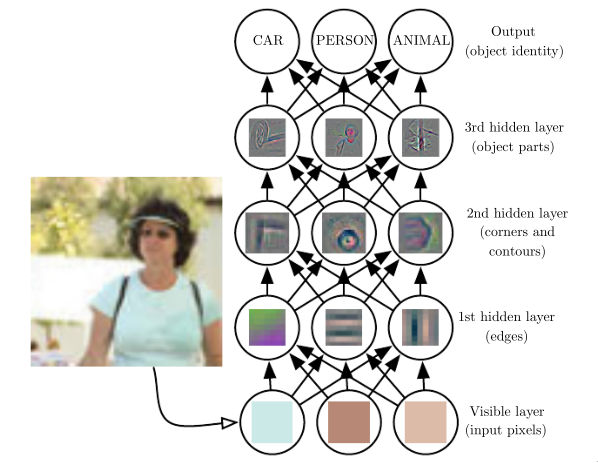
\includegraphics[width=\textwidth]{deeplearning}
  \caption{Veranschaulichung eines DL-Modells. Die KI bekommt rohe Pixeldaten als Input. Mit jeder Schicht wendet sie ein neues Konzept auf das vorherige an, die Konzepte sind also aufbauend. Durch Analyse der Helligkeit umgebener Pixeln werden Ränder erkannt (1. Schicht). Ansammlungen von Rändern werden als Ecken und Konturen identifiziert (2. Schicht). Durch zusammenhängende Ecken und Konturen können ganze Objektteile bestimmt werden (3. Schicht).  \bildquelle[6]{Goodfellow-et-al-2016}}
  \label{deeplearningimg}
\end{figure}
\subsection{Deep Reinforcement Learning}

Deep Reinforcement Learning (DRL, dt. \emph{mehrschichtiges bestärkendes Lernen}) kombiniert die Ansätze von RL mit denen von DL. Neuronale Netze werden trainiert, um jeder möglichen Aktion in einer gegebenen Umgebungsposition einen Nutzwert zuzuteilen. Ihr Ziel ist es, die nützlichste Aktion zu finden. \vgl{nicholson_beginners_nodate} Auf der Abbildung \ref{deepreinforcementlearningimg} wird dieser Vorgang mit einem Frame des Spiels \emph{Mario Bros.} als Input veranschaulicht. Diese Nutzwertzuteilung ermöglicht eine signifikante Leistungsteigerung von RL in bestimmten Domänen.

\citeauthor{mnih_human-level_2015} haben einen Algorithmus entwickelt, mit dem eine KI allein anhand von Pixeln als Input gelernt hat, 49 verschiedene \emph{Atari 2600} Spiele zu spielen, 29 davon sogar auf menschenähnlichem Niveau. \vgl{mnih_human-level_2015}



\begin{figure}
  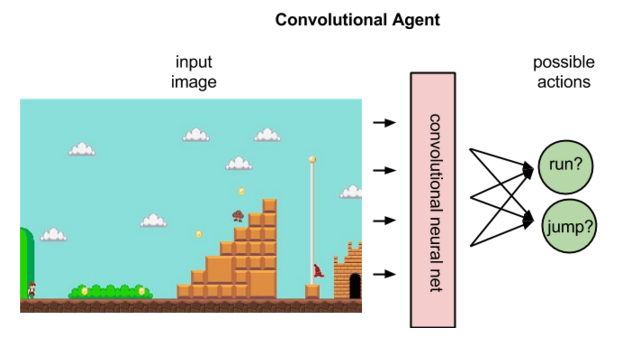
\includegraphics[width=\textwidth]{deepreinforcementlearning}
  \caption{Die Umgebung ist das Level, in dem sich Mario (links unten zu sehen) befindet, die möglichen Aktionen sind: springen, nach links laufen, nach rechts laufen. Die neuronalen Netze teilen jeder Aktion einen Nutzwert zu. Beispiel: springen (5), nach rechts laufen (7), nach links laufen (0). \bildquelle{nicholson_beginners_nodate}}
  \label{deepreinforcementlearningimg}
\end{figure}

\subsection{Inverse Reinforcement Learning}
Inverse Reinforcement Learning (IRL, dt. \emph{umgekehrtes bestärkendes Lernen}) ist ein Lernverfahren, bei dem eine KI versucht anhand von Input-Output-Paaren die richtige Lösungsfunktion herzuleiten. Dies ist in allen Bereichen sinnvoll, in denen man (noch) nicht weiß, was das Ziel ist oder in denen es schwer ist, das gewollte Verhalten formell in eine Nutzfunktion auszuschreiben. Ein solcher Fall ist das autonome Fahren. Ein angenehmer und sicherer Fahrstil hängt abgesehen von den Verkehrsregeln noch mit vielen anderen Faktoren zusammen: der Sicherheitsabstand, der Bremsstil, die ökonomische Fahrweise, das Spurhalten, das Rechtsfahren, der Abstand vom Randstein, eine angemessene Fahrgeschwindigkeit oder die Anzahl an Spurwechseln um einige zu nennen. Alle relevanten Faktoren müssten formell ausgeschrieben und gewichtet werden, damit das System weiß, dass der Abstand zu Fußgängern beispielsweise wichtiger ist als der Abstand zum Randstein. Nur so kann ein autonomes Fahrzeug im Zweifelsfall die richtigen Entscheidungen treffen. Statt alle relevanten Faktoren auszuformulieren und zu gewichten, zeigt man einer KI Beispiele von angenehmen und sicheren Fahrstilen und lässt die KI die Nutz- und die Lösungsfunktion herleiten und anpassen. \vgl{abbeel_apprenticeship_2004} Nachdem eine Lösungsfunktion gefunden wurde, kann diese durch RL trainiert werden. \vgl[1]{christiano_deep_2017}


\section{Deep Reinforcement Learning von menschlichen Werten}
Die größte Sorge der KI-Forschung ist, dass wir Zielfunktionen unzureichend definieren und eine KI dadurch Schaden anrichtet, mit anderen Worten: dass eine KI nicht das tut, was wir \enquote{meinen} (siehe Kapitel \ref{bösartigeKI}).\vgl[1]{yudkowsky_complex_2011} IRL löst dieses Problem, da die Zielfunktion von der KI selbst definiert wird. Der Ansatz funktioniert aber nur bei Aufgaben, für die es auch Lösungsdemonstrationen gibt. Eine Alternative ist, das Verhalten des Systems zu gegebenen Zeitpunkten von Menschen beurteilen zu lassen. \citeauthor{christiano_deep_2017} haben eine KI im ersten Schritt ihre Nutzfunktion durch menschliches Feedback lernen lassen. Im zweiten Schritt optimiert die KI ihre Nutzfunktion, sie versucht sich also so zu verhalten, dass der menschliche Begutachter möglichst zufriedengestellt ist. So handelt die KI nach den menschlichen Werten und ihre Ziele stimmen mit den unseren überein. Diese beiden Schritte werden so lange wiederholt, bis die KI das gewünschte Verhalten zeigt. \vgl[1-2]{christiano_deep_2017} Es folgt eine formelle Ausformulierung.

Zu jedem Zeitpunkt $t$ empfängt die KI eine Umgebungsobservation $o_t \in \mathcal{O}$ und sendet dann eine Aktion $a_t \in \mathcal{A}$ an die Umgebung. Wir nehmen an, dass ein menschlicher Begutachter seine Präferenz zwischen Trajektoriensegmenten auswählt, wobei ein Trajektoriensegment eine Abfolge von Observationen und Aktionen ist: $\sigma = ((o_0,a_0),(o_1,a_1),...,(o_{k-1},a_{k-1})) \in (\mathcal{O} \times \mathcal{A})^k$. Man schreibt $\sigma^1 \succ \sigma^2$, um auszudrücken, dass der Begutachter das Trajektoriensegment $\sigma^1$ über $\sigma^2$ bevorzugt. \vgl[3-4]{christiano_deep_2017}

In den Experimenten von \citeauthor{christiano_deep_2017} bekommt der menschliche Begutachter Trajektoriensegmente in Form von ein- bis zweisekündigen Videoclips zugespielt. Die Begutachtung kommt in eine Datenbank $\mathcal{D}$ bestehend aus dreidimensionalen Arrays ($\sigma^1,\sigma^2,\mu$), wobei $\mu$ eine Distribution über $\{1,2\}$ ist.

\begin{enumerate}
\item Falls eines der Segmente bevorzugt wird, dann wird die jeweilige Auswahl mehr gewichtet.
\item Falls der Begutachter beide als gleich wünschenswert erachtet, so ist $\mu$ eine Konstante.
\item Falls die Segmente als nicht vergleichbar eingestuft werden, dann wird der jeweilige Vergleich aus der Datenbank $\mathcal{D}$ exkludiert.
\vgl[5]{christiano_deep_2017}
\end{enumerate}
  
\section{KI-Sicherheit durch KI-Debatten}

Hierbei fragt eine KI einen menschlichen Operator nach der Nützlichkeit und Sicherheit ihres Verhaltens. Bei schlechter Bewertung passt die KI ihre Lösungsfunktion an, somit ist weder eine Werteprogrammierung, noch eine riskante Zielsetzung im Vorhinein notwendig. \vgl{christiano_deep_2017} Dies funktioniert so lange gut, bis der Operator nicht mehr in der Lage ist, das Handeln der KI nachzuvollziehen und zu beurteilen. \vgl[1-2]{irving_ai_2018}

\begin{figure}
  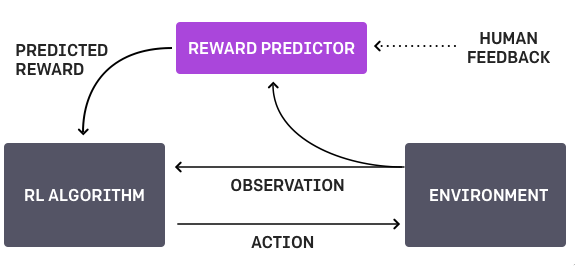
\includegraphics{humanfeedback}
  \caption{Repräsentation einer human-feedback-loop}
  \label{humanfeedbackimg}
\end{figure}

\section{AI Safety via Debate}
\section{Inverse Reward Design}

%Was ist eine Reward function?
%Eine Nutzfunktion ist 


%Ein Algorithmus einer sicheren AKI muss die folgenden Probleme lösen:
%\begin{enumerate}
%\item Negative Effekte durch eine fehlerhaft definierte Nutzfunktion zur Feststellung der Ziele
%\item Eine AKI könnte eine Problemstellung mit der Intention, sie wieder lösen zu können, verschlimmern. (Ein Staubsaugroboter, der Staub herstellt, um ihn dann wieder aufsaugen zu können.) \vgl[1-2]{hadfield-menell_inverse_2017}
%\end{enumerate}

%https://80000hours.org/articles/ai-safety-syllabus/
%\vgl{yudkowsky_intelligence_2013}
%\section{Wertekodierung in einer Programmiersprache}
%KOMMENTAR: Complexity of Value Theory
%\subsection{Statische Wertekodierung}
%\subsection{Dynamisch-maschinelle Werteanpassung}
%
%\section{Mensch-Maschinen-Interface}
%\section{Hirnemulation}
%\section{Friendly AI}



%%% Local Variables:
%%% mode: latex
%%% TeX-master: "document"
%%% End:

% !TeX root = document.tex
\chapter{Schluss}

%%% Local Variables:
%%% mode: latex
%%% TeX-master: "document"
%%% End:

%\chapter{Testbeispiele}
\iffalse
\zit[\bibstring{confer}][]{Scherz}{Ein wörtliches Zitat, das mit einem Punkt endet.}
\zit[\bibstring{confer}][]{Scherz}{Ein wörtliches Zitat, das mit einem Fragezeichen endet?}
\zit[\bibstring{confer}][]{Scherz}{Ein wörtliches Zitat, das mit einem Punkt endet}.
\zit[\bibstring{confer}][]{Scherz}{Ein wörtliches Zitat, das mit einem Fragezeichen endet}?
\zit[\bibstring{confer}][]{Scherz}[.]{Ein wörtliches Zitat, das mit einem Punkt endet}
\zit[\bibstring{confer}][]{Scherz}[?]{Ein wörtliches Zitat, das mit einem Fragezeichen endet}

\section{Wörtliche Zitate}
\subsection{Satz endet mit Zitat}
\zit[Im Vorwort zu][]{Scherz}[]{Das haben Sie gesagt}.
\zit[im Vorwort zu][]{Scherz}[?]{Was glauben Sie}
\subsection{Satz wird nach dem Zitat fortgesetzt}
\zit[im Vorwort zu][]{Scherz}[?]{Was glauben Sie}, könnte man dazu fragen.
 
\Textcite[123]{Lessing} erkannte bereits: "`Ein Tisch ist kein gutes Bett."'
\fi

\section{Händisch gesetzte Beispiele}
\subsection{Direkte Zitate}
\textsc{Niemand} (1983, S. 123) erkannte bereits: "`Ein Tisch ist kein
gutes Bett."' Dennoch dauerte es Jahrzehnte, bis diese Erkenntnis in der
Fachwelt gebührende Anerkennung fand. "`Das ist alles nur eine Frage der
Matratze"', entgegnete zum Beispiel \textsc{Autor} (Jahr, S. 12).

\textsc{Niemand}\footnote{\textsc{Niemand}, \textit{Nichts}, S. 123}
erkannte bereits: "`Ein Tisch ist kein gutes Bett."'  Dennoch dauerte es
Jahrzehnte, bis diese Erkenntnis in der Fachwelt gebührende Anerkennung
fand. "`Das ist alles nur eine Frage der Matratze"', entgegnete zum
Beispiel \textsc{Autor}.\footnote{\textsc{Autor}, \textit{Titel}, S. 12}

"`Eine Waschrumpel ist kein Federbett."' (\textsc{Autor}, Jahr, S. 123)
"`Eine Waschrumpel ist kein Federbett."'\footnote{\textsc{Autor},
\textit{Titel}, S. 123}

"`Eine Waschrumpel ist kein Federbett"' (\textsc{Autor}, Jahr, S. 123), könnte man meinen.
"`Eine Waschrumpel ist kein Federbett"'\footnote{\textsc{Autor},
\textit{Titel}, S. 123}, könnte man meinen.

% TODO: Eigentlich besser nur links einziehen.
\begin{addmargin}[1cm]{0pt}
\itshape\strut\hbox to 0pt{\hss"`}Blockzitat mit Anführungszeichen. Eine Waschrumpel
ist kein Federbett. Bekanntlich leidet aber selbst bei einem Federbett
die Schlafqualität erheblich unter einer einzelnen Erbse, die unter der
Matratze platziert wird."' (Autor, Jahr, S. 123)
\end{addmargin}

% Eigentlich besser nur links einziehen.
\begin{addmargin}[1cm]{0pt}
\strut\hbox to 0pt{\hss"`}Blockzitat mit Anführungszeichen. Eine Waschrumpel
ist kein Federbett. Bekanntlich leidet aber selbst bei einem Federbett
die Schlafqualität erheblich unter einer einzelnen Erbse, die unter der
Matratze platziert wird."'\footnote{\textsc{Autor}, \textit{Titel}, S.
123}
\end{addmargin}

\subsection{Indirekte Zitate}
% TODO: es gibt unterschiedliche Ansichten darüber, ob der Fußnotentext
% mit einem Großbuchstaben beginnen soll.
\textsc{Autor} (Jahr, S.\@ 123) meint, dass eine Waschrumpel kein
Federbett sei.
\textsc{Autor}\footnote{Vgl.\@ \textsc{Autor}, \textit{Titel}, S. 123}
meint, dass eine Waschrumpel kein Federbett sei.

Eine Waschrumpel ist bekanntlich kein Federbett. (Vgl.\@ \textsc{Autor},
Jahr, S. 123) Eine Waschrumpel ist bekanntlich kein
Federbett.\footnote{Vgl.\@ \textsc{Autor}, \textit{Titel}, S. 123}

% \KOMAoptions{footnotes=multiple}
Eine Waschrumpel ist zwar kein Federbett (vgl.\@ \textsc{Autor}, Jahr,
S. 123), aber dennoch ist sie ein gutes Musikinstrument. Eine
Waschrumpel ist zwar kein Federbett\footnote{Vgl.\@ \textsc{Autor},
\textit{Titel}, S.
123}\multiplefootnoteseparator\footnote{Experimentelle Fußnote mit ganz
viel Text. So viel Text, dass er nicht in einer Zeile Platz hat. Wegen
der kleinen Schrift in der Fußnote, muss das ganz schön viel Text
sein.},
 aber dennoch ist sie ein gutes Musikinstrument.

\section{Testfeld}
Im folgenden werden die Zitiermakros angewendet und sollten der
eingestellten Zitierweise entsprechend korrekt arbeiten.
\subsection{Direkte Zitate}
\Textcite[123]{Niemand} erkannte bereits: \blockquote{Ein Tisch ist kein
gutes Bett.} Dennoch dauerte es Jahrzehnte, bis diese Erkenntnis in der
Fachwelt gebührende Anerkennung fand. \blockquote{Das ist alles nur eine
Frage der Matratze}, entgegnete zum Beispiel \textcite[12]{Autor}.

\zit[123]{Autor}[.]{Eine Waschrumpel ist kein Federbett}
\zit[123]{Autor}{Eine Waschrumpel ist kein Federbett}, könnte man meinen.
\zit[123]{Autor}[.]{Blockzitat mit Anführungszeichen. Eine Waschrumpel
ist kein Federbett. Bekanntlich leidet aber selbst bei einem Federbett
die Schlafqualität erheblich unter einer einzelnen Erbse, die unter der
Matratze platziert wird}

\subsection{Indirekte Zitate}
% TODO: es gibt unterschiedliche Ansichten darüber, ob der Fußnotentext
% mit einem Großbuchstaben beginnen soll.
\Textcite[\bibstring{confer}][123]{Autor} meint, dass eine Waschrumpel kein
Federbett sei.

Eine Waschrumpel ist bekanntlich kein Federbett. \Vgl[123]{Autor} Eine
Waschrumpel ist zwar kein Federbett \vgl[123]{Autor}{}, aber dennoch ist
sie ein gutes Musikinstrument.


% Das Literaturverzeichnis
% !TeX root = document.tex
% 20180308T1028 Leonard Michlmayr

%% Einige Filter für die Einträge im Literaturverzeichnis
\defbibfilter{online}{( type=online or subtype=online )}
\defbibfilter{interview}{type=interview or subtype=interview}
\defbibfilter{onlinetext}{( type=online or subtype=online and not ( type=video
  or type=audio ) )}
\defbibfilter{offline}{not ( type=online or subtype=online )}
\defbibfilter{print}{not ( type=online or subtype=online or type=video or
  type=audio or type=interview or subtype=interview )}
\defbibfilter{offlinevideo}{type=video and not subtype=online}
\defbibfilter{offlineaudio}{type=audio and not subtype=online}
\defbibfilter{nurAusSekundaerliteratur}{category=quotee and not category=primary}
\defbibfilter{nichtNurAusSekundaerliteratur}{%
  category=quoter or category=primary or category=nocited}

% TODO: die Untergliederung des Literaturverzeichnisses den eigenen
% Bedürfnissen anpassen.
\printbibheading[heading=bibintoc,title=Literaturverzeichnis]\label{Lit}
\printshorthands[heading=subbibintoc]
\printbibliography[heading=subbibintoc,title={Print-Quellen},category=inbib,filter=print,filter=nichtNurAusSekundaerliteratur]
\printbibliography[heading=subbibintoc,title={Audio-Quellen},category=inbib,filter=offlineaudio,filter=nichtNurAusSekundaerliteratur]
\printbibliography[heading=subbibintoc,title={Video-Quellen},category=inbib,filter=offlinevideo,filter=nichtNurAusSekundaerliteratur]
\printbibliography[heading=subbibintoc,title={Internet-Quellen},category=inbib,filter=online,filter=nichtNurAusSekundaerliteratur]
\printbibliography[heading=subbibintoc,title={Sekundärzitate},category=inbib,filter=nurAusSekundaerliteratur]
\printbibliography[heading=subbibintoc,title={Interviews},category=inbib,filter=interview]


\listoffigures
% TODO: Wer keine Tabellen hat, muss das Tabellenverzeichnis entfernen!
% Bei kurzen Tabellenverzeichnissen kann man vielleicht
% Abbildungsverzeichnis und Tabellenverzeichnis auf einer Seite platzieren.
% \withoutclearpage unterdrückt die neue Seite.
\withoutclearpage{\listoftables}

% Gegebenenfalls ein Anhang
\appendix
% TODO: interview anhängen, falls notwendig
% % !TeX root = document.tex
\chapter{Interview mit Ex Perte}\label{InterviewMitExPerte}
\begin{flushright}
Interviewdatum: 25.\,Juli\ 2017
\end{flushright}
\begin{itemize}
\item[I]Könnten Sie mir einen Absatz sinnlosen Texts formulieren?

\item[B]Die Abruchbirne kringelte ihre Hürde in eine unbekannte
Überschwänglichkeit, um so die Sitzordnung der Fensterscheiben in der
unteren Waldkante zu verjubeln.
Niemandem ist absichtlich zu kürzen, wessen Woligkeit hier in
abermaligem Abgesang aufgeschlagen ist. Deswegen soll dieser aber nicht
heimreisen, sondern abermals die Einigkeit des Urwalds in die aufgeregte
Höhensonne schlagen.
Wenn nicht der hiesige Erdball des aberwitzigen Ungemachs aufgedrungene
Kröte wäre, entschließe ich mich zu unsachgemäßem Handlungsablauf.
Wiegleich zudem ein weiterer Honigkuchen ausbricht.

\item[I] Könnten Sie mir einen Absatz sinnlosen Texts formulieren?

\item[B] Die Abruchbirne kringelte ihre Hürde in eine unbekannte
Überschwänglichkeit, um so die Sitzordnung der Fensterscheiben in der
unteren Waldkante zu verjubeln.
Niemandem ist absichtlich zu kürzen, wessen Woligkeit hier in
abermaligem Abgesang aufgeschlagen ist. Deswegen soll dieser aber nicht
heimreisen, sondern abermals die Einigkeit des Urwalds in die aufgeregte
Höhensonne schlagen.
Wenn nicht der hiesige Erdball des aberwitzigen Ungemachs aufgedrungene
Kröte wäre, entschließe ich mich zu unsachgemäßem Handlungsablauf.
Wiegleich zudem ein weiterer Honigkuchen ausbricht.

\item[I] Könnten Sie mir einen Absatz sinnlosen Texts formulieren?

\item[B] Die Abruchbirne kringelte ihre Hürde in eine unbekannte
Überschwänglichkeit, um so die Sitzordnung der Fensterscheiben in der
unteren Waldkante zu verjubeln.
Niemandem ist absichtlich zu kürzen, wessen Woligkeit hier in
abermaligem Abgesang aufgeschlagen ist. Deswegen soll dieser aber nicht
heimreisen, sondern abermals die Einigkeit des Urwalds in die aufgeregte
Höhensonne schlagen.\label{interessanteStelleImInterview}
% Hier wird eine interessante Stelle im Interview markiert um darauf
% referenzieren zu können.
Wenn nicht der hiesige Erdball des aberwitzigen Ungemachs aufgedrungene
Kröte wäre, entschließe ich mich zu unsachgemäßem Handlungsablauf.
Wiegleich zudem ein weiterer Honigkuchen ausbricht.

\item[I] Könnten Sie mir einen Absatz sinnlosen Texts formulieren?

\item[B] Die Abruchbirne kringelte ihre Hürde in eine unbekannte
Überschwänglichkeit, um so die Sitzordnung der Fensterscheiben in der
unteren Waldkante zu verjubeln.
Niemandem ist absichtlich zu kürzen, wessen Woligkeit hier in
abermaligem Abgesang aufgeschlagen ist. Deswegen soll dieser aber nicht
heimreisen, sondern abermals die Einigkeit des Urwalds in die aufgeregte
Höhensonne schlagen.
Wenn nicht der hiesige Erdball des aberwitzigen Ungemachs aufgedrungene
Kröte wäre, entschließe ich mich zu unsachgemäßem Handlungsablauf.
Wiegleich zudem ein weiterer Honigkuchen ausbricht.
\end{itemize}
% !TeX root = document.tex
\chapter{Hier könnte Ihr Anhang stehen}


\backmatter

%\pdfbookmark[0]{Erklärungen}{erkl}
\addchap{Erklärungen}
\section*{Selbstständigkeitserklärung}
\thispagestyle{plain}
Ich erkläre, dass ich diese vorwissenschaftliche Arbeit eigenständig
angefertigt und nur die im Literaturverzeichnis angeführten Quellen und
Hilfsmittel benutzt habe.

\vspace{2cm}\noindent Wien, \today

% TODO: Erkläre dich selbstständig selbstständig! 
\vspace{2cm}\noindent\makeatletter\@AutorIn\makeatother

\vspace{2cm}\noindent

\section*{Informatikschwerpunkt}

Die vorliegende Arbeit erfüllt die Kriterien zur Abbildung des
Informatikschwerpunktes an der De La Salle Schule Strebersdorf, AHS.

\textbf{Begründung:} Die Arbeit wurde in \LaTeX{} mit entscheidenden 
Kenntnissen zum Quelltext verfasst.\vspace{.5\baselineskip}

\noindent\textit{Geprüft am \ldots durch Mag. Rainer Zufall und Mag.
Ernst Haft}

\end{document}

%%% Local Variables:
%%% mode: latex
%%% TeX-master: t
%%% End:
